\chapter{Design}

\section{User Context}
During the authentication process, the crucial part to successfully authenticate user is to get information about multiple authentication factors, as described in the section \ref{authentication-factors}.
It is an essential part of security strengthening as the more information we get from the authentication attempt, the more we can react to it and evaluate it.

User context is a concept that represents a piece of information about the authentication attempt, such as current device attributes, information about the user, location, or behavior we detected.
Even though the information about the device does not seem to reflect the term user context, it should be considered like it.
User context represents the information about the user of the application, even when it is a service account, for instance.

During the authentication process, user contexts are always collected and grouped into a more comprehensive knowledge base.
The proper user context management is a crucial part of the authentication, especially for the risk-based authentication mechanism.

The abstraction around fetching user contexts provides the ability to easily extend and process possible user context information and gives the freedom to obtain various types of contexts, even from remote locations.

The main advantage of using user contexts is to get the required information, regardless of the source of the information.
It means that it does not really matter which approach was used for obtaining the information, but that the information is available.
It implies that administrators need to be aware of present user context providers/implementations in order to prevent any inaccuracies.

\subsection{Specific User Context}
An excellent example of leveraging user context is the implementation of an IP address context.
It provides the ability to obtain the IP address of the device in multiple ways.
The IP address can be obtained either from the user agent attributes or from the HTTP headers 'Forwarded' and 'X-Forwarded-For' when a proxy is used.
// TODO add diagrams

\subsection{User Context Condition}
Improvement to the user context management is to have a general concept for evaluating certain conditions with regard to the user context.
It means that we can leverage user context conditions in conditional authentication flows or in authentication policies, as described in \ref{authentication-policies}.

There might be several possible operations on the user context entities, and the developer of the additional user context should not reinvent the wheel around attributes of conditions.
The additional conditions can be created very easily, as the general concept for evaluating them has already been assessed.

\subsubsection{Operations}
User context conditions take into account a list of operations that can be proceeded on the user context entity.
The operation consists of several attributes, such as follows:

\begin{itemize}
    \item \textbf{Symbol} (\textit{string}) -- unique operation identifier used for identification of the operation when serialized data are received from remote locations. It must be unique per the user context condition.
    \item \textbf{Text} (\textit{string}) -- name of the operation shown to the end user.
    It can contain a localization key, which can then be mapped to a different language or directly the text in the specific language. 
    \item \textbf{Predicate} (\textit{predicate}) -- predicate that is applied to the specific user context. When the evaluation of the predicate is met, the operation is considered successful.
\end{itemize}

When all the predicates of specified operations are met, the whole condition is considered successful, and the authentication flow can proceed with the processing.

\subsubsection{Example}

A suitable example of the user context condition might be a newly introduced condition for the IP address user context entity.
During the evaluation of the condition, the first step is obtaining the IP address context, which contains the current IP address of the device that is trying to authenticate.
Some specified operations that can be made on top of the IP address context are `is equal`, `is not equal` or `is in range`.

The predicate of the \textit{equal} operation is to directly match the IP address provided by the administrator.
The opposite \textit{not equal} operation just negatively matches the IP address, as it represents the state when the IP address is not the specified one.
Administrators can also specify the `in range` operation, which provides the ability to check whether the IP address of the device is in the specified IP address range.

For instance, an administrator can specify that IP addresses from the range `222.0.0.0-224.0.0.0` are not allowed to be authenticated, as shown in Figure \ref{fig:design-user-context-ip-addr-condition}.

\begin{figure}[htbp]
  \centering
  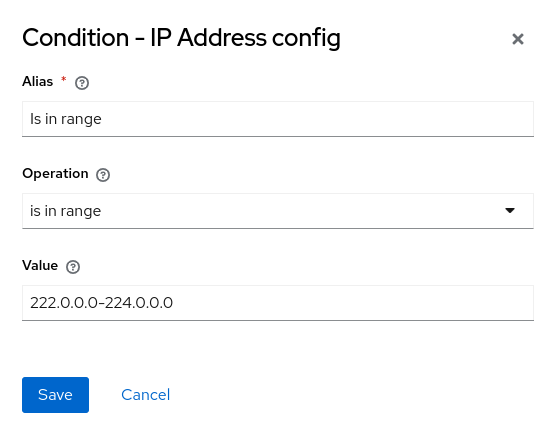
\includegraphics[width=0.8\textwidth]{img/sections/5-design/ip-address-condition.png}
  \label{fig:design-user-context-ip-addr-condition}
  \caption{IP address context condition}
\end{figure}

// TODO add diagrams with operations

\section{Authentication Policies} \label{authentication-policies}
Design of the Authentication policies, or as described in the specification as a Policy engine, provides the ability to comply with requirements specified by the administrator.
When users are trying to access the application, they need to meet certain conditions in order to achieve a successful login.
There may be some company or federal restrictions to particular services that need to be conformed to.

For instance, there might be some requirements to deny users access to the application from a specific country or specific types of devices.

It needs to be determined in which authentication process phases these policies should be evaluated.
Policies might be required to comply with some preconditions in order to be able to evaluate them.
It means that the environment context needs to be aligned with the policy requirement, such as gathering information about the user attempting to log in.

A particular hierarchy in policy priorities needs to be assessed as well in order to evaluate specific policies before others.
It provides the capability to create a more complex and comprehensive evaluation pipeline for authentication policies.

Every authentication policy consists of several conditions and actions.
All conditions must be met in order to execute specific actions.
If some of these conditions are not evaluated to be true, the whole authentication policy is skipped, and the following policy in the hierarchy structure is evaluated.

Authentication policies can be specified interactively via the administrator console or HTTP REST API.
All of them are stored in persistent storage, so every change of the structure is visible even after the re-initialization of the application. 
Specific operations can be executed on the policy entities, such as obtaining a specific authentication policy, creating a new one, or updating or removing the existing one.
Moreover, the priority to achieve the required hierarchy structure can be defined as well.

\subsection{Authentication Flow}

Authentication policies are tightly coupled to the authentication flows described in the section \ref{keycloak-authentication-flows}.
Authentication policies are a specific subset of authentication flows as these policies are basically just conditional authentication flows.

Conditional flows provide the majority of the required functionality to meet requirements for authentication policies or the policy engine.
It means that specific conditions are evaluated, and if all pass, specific actions are executed.

One of the major issues around authentication policies is manageability.
Administrators should not add a higher number of conditional flows to their existing authentication flows, as these concepts should be separated in this manner.

Authentication policies extend the capabilities around the authentication flow process as they can be defined for the whole realm, not even for a specific flow.
To be more specific, it gives the possibility to share policies across different flows, which is the main difference between conditional flows and authentication policies.

It provides more fine-grained authentication policy management and a better authentication settings approach.

\subsection{Authentication Policy Authenticator}
In order to properly evaluate all authentication policies specified for the realm without the need to comprehensively expand the authentication flows, a specific authenticator was introduced.
It provides the ability to have a more fine-grained approach for these evaluations, as the administrator can specify in which phases of the authentication flow these policies will be processed.

The authenticator works as a configurable placeholder for these policies, as it can contain multiple configuration properties to asses the overall policies processing.
It might be possible to hide the authenticator from the flows completely, but the explicit settings provide a more deterministic approach.

The default authenticator configuration contains only a boolean flag to determine whether the user information is required for the evaluations or not.

When the authentication flow processing is in the phase of evaluating the authenticator, multiple steps are executed:

\begin{enumerate}
    \item \textbf{Obtain} -- Obtain all authentication policies.
    \item \textbf{Filter} -- Filter policies based on the authenticator configuration.
    \item \textbf{Process} -- Process all authentication policies.
    \item \textbf{Return} -- Return to the parent authentication flow and continue with processing other steps.
\end{enumerate}

When all conditions are met for an arbitrary policy, and the action explicitly allows access to the user, the authenticator itself is evaluated as successful without any other policy evaluations.

The same applies to the case when the action explicitly denies access to the user, the authenticator is evaluated as false, and the whole authentication flow processing is stopped.

Otherwise, when the action is not terminal, the other policies are evaluated as usual.

\subsection{Administrator Console}
// TODO add screenshots of admin pages and elaborate on them

\subsection{Policy Evaluation Example}
For a better representation of the authentication policy evaluation, a simple example with the described configuration might be considered.
The specification of a particular authentication policy is done through the administrator console in the Authentication section and Authentication Policies tab.

The following simple example of the authentication policy, in figure \ref{fig:design-policy-browser-flow}, has one condition and one action.
If the first condition is met, the underlying action is executed.

The policy contains a condition based on the current browser properties, which does not allow a specific browser vendor - Mozilla Firefox, in this case.
When the condition is met, access to the application is denied to the user.
This means that authentication requests can only be made via a browser other than Mozilla Firefox.

\begin{figure}[htbp]
  \centering
  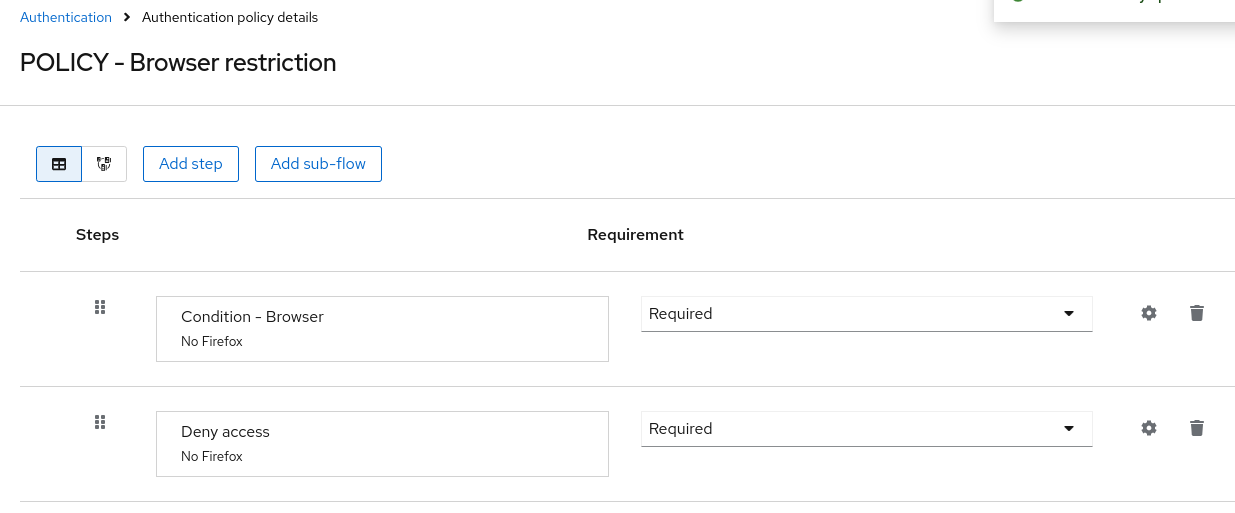
\includegraphics[width=1\textwidth]{img/sections/5-design/policy-browser-flow.png}
  \label{fig:design-policy-browser-flow}
  \caption{Authentication policy browser restriction}
\end{figure}

For a better visualization of the condition evaluation flow, consider this diagram:

\begin{figure}[htbp]
  \centering
  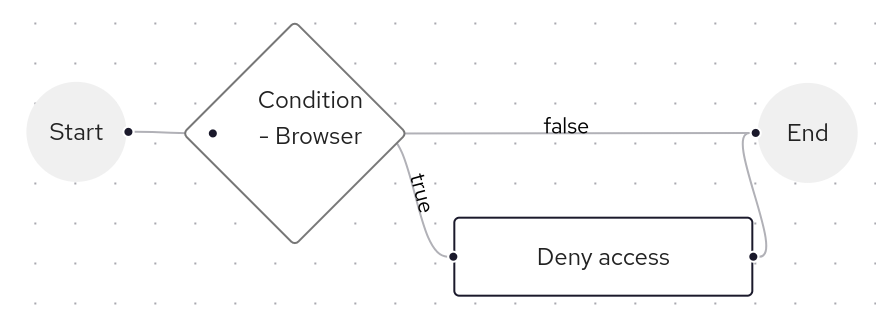
\includegraphics[width=0.8\textwidth]{img/sections/5-design/policy-browser-flow-graph.png}
  \label{fig:design-policy-browser-flow-graph}
  \caption{Authentication policy browser restriction graph}
\end{figure}

The condition configuration attributes differ based on the used condition provider/implementation.
Every condition provider specifies a set of configuration properties for condition settings.

The browser condition, shown in Figure \ref{fig:design-policy-browser-flow-condition}, includes properties:

\begin{itemize}
    \item \textbf{Alias} -- name of the condition.
    \item \textbf{Operation} -- list of possible operations.
    \item \textbf{Browser} -- multi valued list of browsers. 
\end{itemize}

In this case, the condition is met only when the browser vendor is Firefox:

\begin{figure}[htbp]
  \centering
  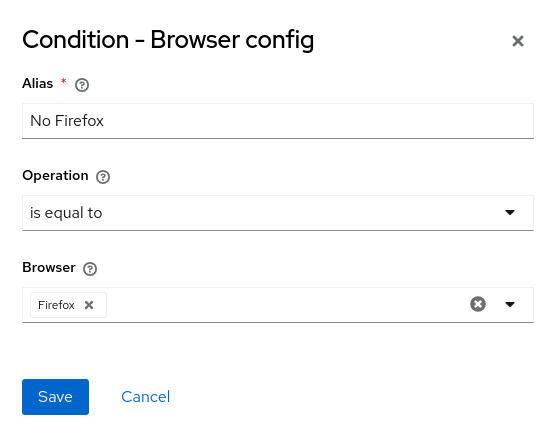
\includegraphics[width=0.8\textwidth]{img/sections/5-design/policy-browser-condition.png}
  \label{fig:design-policy-browser-flow-condition}
  \caption{Browser restriction condition}
\end{figure}

The action configuration also differs based on the provider of the action.
For the Deny access provider, visible in Figure \ref{fig:design-policy-browser-flow-deny}, the only additional property is \textit{Error Message}.
It represents an error message that is shown to the user when the access is denied.

\begin{figure}[htbp]
  \centering
  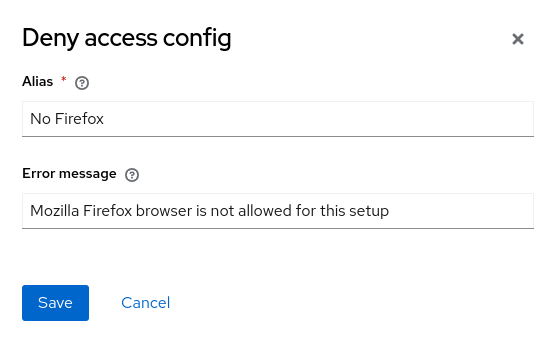
\includegraphics[width=0.8\textwidth]{img/sections/5-design/policy-browser-deny.png}
  \label{fig:design-policy-browser-flow-deny}
  \caption{Browser restriction deny access}
\end{figure}

\newpage
\section{Risk-based Authentication}
The crucial part of adaptive authentication is focused on risk-based authentication.
Risk-based authentication is a concept that assesses a risk level and then adjusts authentication requirements accordingly.
The risk in the risk-based authentication represents a probability that the authentication attempt is fraudulent.
\newline
\newline
The concept is based on this core sequence:
\begin{enumerate}
    \item \textbf{User Context Collection} -- Gather all available user contexts for the following processing. 
    \item \textbf{Risk scoring} -- Assess the risk score for all the user contexts. 
    \item \textbf{Adaptive adjustment} -- Adaptively adjust authentication flow based on the overall risk score.
\end{enumerate}

The collection of user contexts is an essential part of the whole risk-based authentication concept - as more information is present, the more informed decisions can be made.
There is a defined timeout for obtaining the user context, as it may take a vast majority of time, and administrators are able to adjust it to their needs.

Obtaining user context from remote locations or services may be time-consuming, and the overall user experience around the authentication process would be worse.
When the timeout is exceeded, the user context is not taken into account for the risk evaluation.

When the user context collection is successful, the risk is evaluated for every user context.
The exact approach and how it is achieved is described in \ref{risk-evaluators}.

When all these evaluations are done, the overall risk for the authentication attempt is calculated with the usage of various algorithms described in \ref{risk-engine}.

After calculating the overall risk, the risk level is determined based on the risk score, described in \ref{risk-levels}.

\subsection{Risk Evaluators} \label{risk-evaluators}
\subsection{Risk Engine} \label{risk-engine}
\subsection{Risk Levels} \label{risk-levels}
\subsection{Risk Level conditions}


\section{Artificial Intelligence}


\section{External Integration}